\documentclass[frenchb, oneside, headings=normal]{scrartcl}

\usepackage[utf8x]{inputenc}
\usepackage[T1]{fontenc}
\usepackage{lmodern}

\usepackage{ifthen}
\usepackage{url}


\usepackage{multirow}

% Color
% cfr http://en.wikibooks.org/wiki/LaTeX/Colors
\usepackage{color}
\usepackage[usenames,dvipsnames,svgnames,table]{xcolor}
\definecolor{dkgreen}{rgb}{0.25,0.7,0.35}
\definecolor{dkred}{rgb}{0.7,0,0}

\newcommand{\matlab}{\textsc{Matlab}}

% Math symbols
\usepackage{amsmath}
\usepackage{amssymb}
\usepackage{amsthm}
\DeclareMathOperator*{\argmin}{arg\,min}
\DeclareMathOperator*{\argmax}{arg\,max}


% Sets
\newcommand{\Z}{\mathbb{Z}}
\newcommand{\R}{\mathbb{R}}
\newcommand{\Rn}{\R^n}
\newcommand{\Rnn}{\R^{n \times n}}
\newcommand{\C}{\mathbb{C}}
\newcommand{\K}{\mathbb{K}}
\newcommand{\Kn}{\K^n}
\newcommand{\Knn}{\K^{n \times n}}

% Unit vectors
\usepackage{esint}
\usepackage{esvect}
\newcommand{\kmath}{k}
\newcommand{\xunit}{\hat{\imath}}
\newcommand{\yunit}{\hat{\jmath}}
\newcommand{\zunit}{\hat{\kmath}}
\newcommand{\uunit}{\hat{\umath}}

% rot & div & grad & lap
\DeclareMathOperator{\newdiv}{div}
\newcommand{\divn}[1]{\nabla \cdot #1}
\newcommand{\rotn}[1]{\nabla \times #1}
\newcommand{\grad}[1]{\nabla #1}
\newcommand{\gradn}[1]{\nabla #1}
\newcommand{\lap}[1]{\nabla^2 #1}


% Elec
\newcommand{\B}{\vec B}
\newcommand{\E}{\vec E}
\newcommand{\EMF}{\mathcal{E}}
\newcommand{\perm}{\varepsilon} % permittivity

\newcommand{\bigoh}{\mathcal{O}}
\newcommand\eqdef{\triangleq}

\DeclareMathOperator{\newdiff}{d} % use \dif instead
\newcommand{\dif}{\newdiff\!}
\newcommand{\fpart}[2]{\frac{\partial #1}{\partial #2}}
\newcommand{\ffpart}[2]{\frac{\partial^2 #1}{\partial #2^2}}
\newcommand{\fdpart}[3]{\frac{\partial^2 #1}{\partial #2\partial #3}}
\newcommand{\fdif}[2]{\frac{\dif #1}{\dif #2}}
\newcommand{\ffdif}[2]{\frac{\dif^2 #1}{\dif #2^2}}
\newcommand{\constant}{\ensuremath{\mathrm{cst}}}

\usepackage{siunitx}

\usepackage{tikz}

\usepackage{pgfplots}
\usepackage{lmodern}
\usepackage{microtype}
\usepackage{xspace}

\usepackage{babel}
% Listing
% always put it after babel
% http://tex.stackexchange.com/questions/100717/code-in-lstlisting-breaks-document-compile-error
\usepackage{listings}

\definecolor{mygreen}{rgb}{0,0.6,0}
\definecolor{mygray}{rgb}{0.5,0.5,0.5}
\definecolor{mymauve}{rgb}{0.58,0,0.82}
\lstset{ %
  language=Matlab,
  backgroundcolor=\color{white},   % choose the background color; you must add \usepackage{color} or \usepackage{xcolor}
  basicstyle=\footnotesize,        % the size of the fonts that are used for the code
  breakatwhitespace=false,         % sets if automatic breaks should only happen at whitespace
  breaklines=true,                 % sets automatic line breaking
  captionpos=b,                    % sets the caption-position to bottom
  commentstyle=\color{mygreen},    % comment style
  deletekeywords={...},            % if you want to delete keywords from the given language
  escapeinside={\%*}{*)},          % if you want to add LaTeX within your code
  extendedchars=true,              % lets you use non-ASCII characters; for 8-bits encodings only, does not work with UTF-8
  frame=single,	                   % adds a frame around the code
  keepspaces=true,                 % keeps spaces in text, useful for keeping indentation of code (possibly needs columns=flexible)
  keywordstyle=\color{blue},       % keyword style
  otherkeywords={*,...},           % if you want to add more keywords to the set
  numbers=none,                    % where to put the line-numbers; possible values are (none, left, right)
  numbersep=5pt,                   % how far the line-numbers are from the code
  numberstyle=\tiny\color{mygray}, % the style that is used for the line-numbers
  rulecolor=\color{black},         % if not set, the frame-color may be changed on line-breaks within not-black text (e.g. comments (green here))
  showspaces=false,                % show spaces everywhere adding particular underscores; it overrides 'showstringspaces'
  showstringspaces=false,          % underline spaces within strings only
  showtabs=false,                  % show tabs within strings adding particular underscores
  stepnumber=2,                    % the step between two line-numbers. If it's 1, each line will be numbered
  stringstyle=\color{mymauve},     % string literal style
  tabsize=2,	                   % sets default tabsize to 2 spaces
  title=\lstname                   % show the filename of files included with \lstinputlisting; also try caption instead of title
}

\KOMAoptions{DIV=last}

\usepackage[top = 2.5 cm, bottom = 3 cm, left = 2.5 cm, right = 2.5 cm]{geometry}
\usepackage{caption}


\usepackage{epstopdf}
\usepackage{wrapfig}
\usepackage{verbatim}
\begin{document}

\title{Projet ELEC Master 1 - Labo 6}
\subtitle{Groupe 4}
\author{Deprez Damien \and Bilal Ouachalih }
\date{2 december 2016}
\maketitle

The purpose of this lab is to study the OFDM (\textit{\textbf{orthogonal frequency division multiplexing}}) modulation. An interpretation is that OFDM devides a frequency selective channel into N flat fadding subchannels. We can see that as N parallel flat fadding channels multiplexed in the frequency domain. The cyclic prefix is used to avoid intersymbol interference (\textbf{ISI}).

\begin{figure}[!ht]
\centering
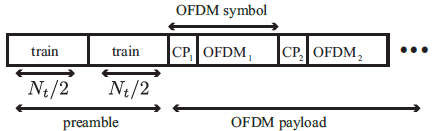
\includegraphics[scale=0.8]{img/operation_ofdm.png}
\caption{Representation of what's being done by the OFDM modulation}
\label{fig1}
\end{figure}

\section{Pre-lab}

In the first part of the lab, we have implemented an OFDM modulator  and the corresponding demodulator. First, at the transmitter side

\begin{itemize}

\item We have a sequence of $N-K$ symbols where N is the number of subcarriers and K is the number of null subcarrier.

\item \textbf{Null symbols} are inserted into groups of $N-K$ transmit suymbols.

\item We have an \textbf{IFFT} of the previous symbols.

\item Then, a \textbf{cyclic prefix} of length $L_c$ is added at the transmitter.

\end{itemize}

Second, at the receiver side

\begin{itemize}

\item The receiver consider block of $N+L_c$ without regarding the first $L_c$ samples of each block.

\item Then, we take back the \textbf{FFT} of the N symbols.

\end{itemize}

This previous 'operations' are represented on the block diagam on the figure \ref{fig2} and \ref{fig3}.

\begin{figure}[!ht]
    \begin{minipage}[b]{0.48\linewidth}
        \centering 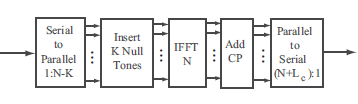
\includegraphics[scale=0.9]{img/OFDDM_modulator.png}
     \caption{Block diagram of the OFDM modulator}
     \label{fig2}
    \end{minipage}\hfill
    \begin{minipage}[b]{0.48\linewidth}
         \centering 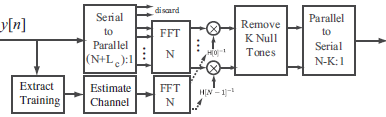
\includegraphics[scale=0.9]{img/OFDDM_demodulator.png}
 \caption{Block diagram of the OFDM demodulator}\label{fig3}
    \end{minipage}
\end{figure}

\section{Lab experiment}

\subsection{What is the respective OFDM symbol rate in the narrowband and wideband systems you have set up ?}

For $N=64$, and $L_c=8$

\begin{center}
	\begin{tabular}{c|c|c}
		  & Narrowband & Wideband\\
		  \hline
	Tx Sample rate & 4 $MSample/s$ & 20 $MSample/s$ \\	  
	Tx Oversample factor & 20 & 4\\
	\textbf{ODFM symbol rate} &  $\textbf{2777.77 symbol/s}$ & $\textbf{69444.44 symbol/s}$ \\ 
	\end{tabular}
	\label{tab1}
\end{center}

We simply have calculated the OFDM symbol rate by using the following formula

\begin{equation}
OFDM~symbol~rate = \frac{Tx~sample~rate}{(N+L_c)*Tx~oversample~factor}
\end{equation}

We can directly see that the symbol period is greater in a narrowband channel the in an wideband channel. (important for the future question). 

\subsection{What are the effective lengths of the narrowband and wideband channels respectively?}

If we take a look on the figure \ref{fig4} and \ref{fig5} representing the power delay in both case (narrow and wideband channel), we can deduce the effective length of the channel. The effective length are of $\textbf{2.5e-7~s}$ and $\textbf{1e-7~s}$ respectively for the narrowband and wideband channel.

\begin{figure}[!ht]
    \begin{minipage}[b]{0.48\linewidth}
        \centering 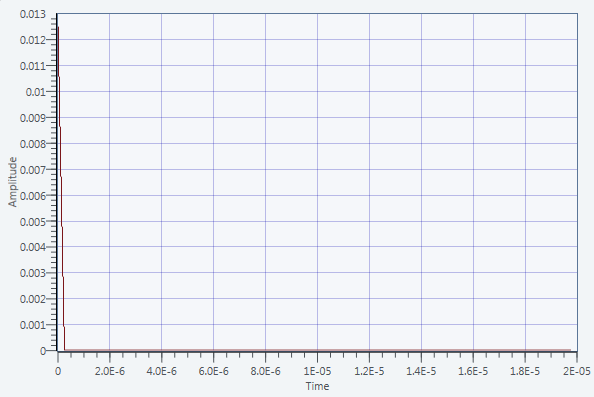
\includegraphics[scale=0.45]{img/power_delay_narrow.png}
     \caption{Power delay of the narrowband channel}
     \label{fig4}
    \end{minipage}\hfill
    \begin{minipage}[b]{0.48\linewidth}
         \centering 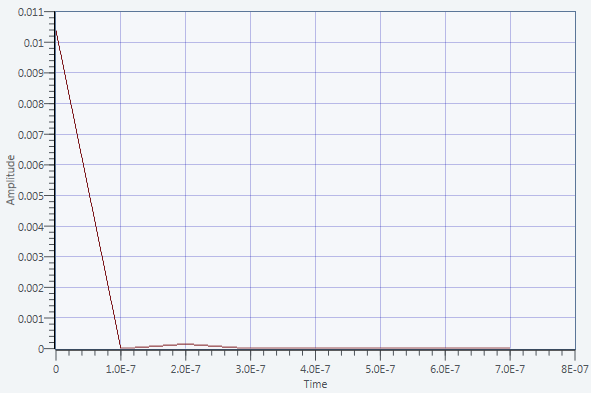
\includegraphics[scale=0.45]{img/power_delay_wideband.png}
 \caption{Power delay of the wideband channel}\label{fig5}
    \end{minipage}
\end{figure}
\subsection{Describe the frequency responses of each channel.}

\begin{figure}[!ht]
    \begin{minipage}[b]{0.48\linewidth}
        \centering 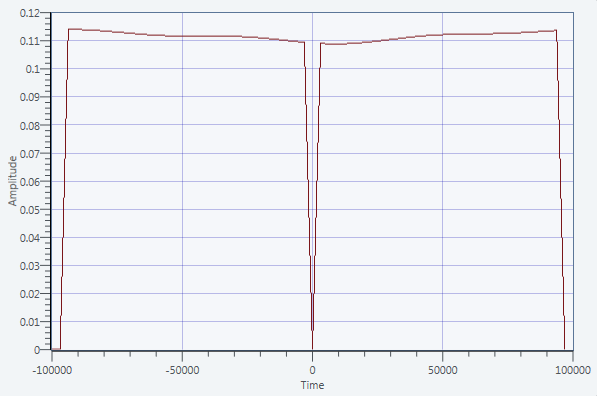
\includegraphics[scale=0.45]{img/channel_response_narrow.png}
     \caption{Response of a narrowband channel}
     \label{fig2}
    \end{minipage}\hfill
    \begin{minipage}[b]{0.48\linewidth}
         \centering 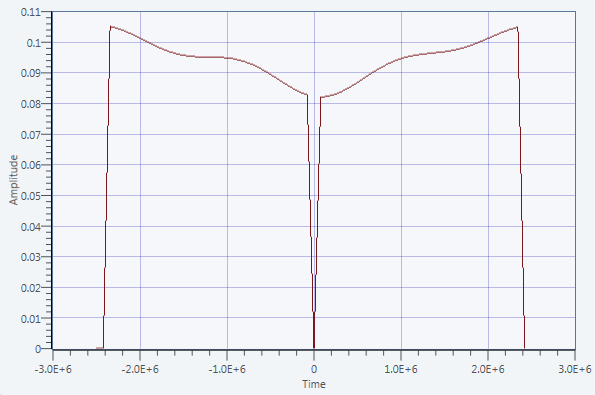
\includegraphics[scale=0.45]{img/channel_response_wideband.png}
 \caption{Response of a wideband channel}\label{fig3}
    \end{minipage}
\end{figure}

\begin{comment}
We can characterize a flat or a frequency-selective channel by comparing the bandwidth of the signal with the bandwidth of the channel (or the symbol period and the effective length).\\

\begin{itemize}
\item For a flat channel, we have that \textbf{Bandwidth of channel > Bandwidth of the symbol}.
\item For a frequency-selective channel, we have just the inverse, \textbf{Bandwidth of channel < Bandwidth of the symbol}. 

\end{itemize}
\end{comment}

By using the value computed in the previous question, we can deduce that

\begin{center}
	\begin{tabular}{c|c|c}
		  & Narrowband & Wideband\\
		  \hline
	Tx Sample rate & 4 $MSample/s$ & 20 $MSample/s$ \\	  
	Tx Oversample factor & 20 & 4\\
	\hline
     & \color{red} \textbf{Flat}  & \color{red} \textbf{Frequency-selective}\\                               
	\end{tabular}
	\label{tab1}
\end{center}
%TODO {Question sur frequency-selective channel}
Based on our observation of graph \ref{fig3} and \ref{fig4}, we see that the frequency response in narrowband is flat, because we have only one peak on the graph of the power delay, but in wideband channel, we have 2 peaks on the power delay, which tell us that it's frequency-selective.
Another thing we can see from the channel response, is that we have a big attenuation at $0 Hz$. Which means that the zero frequency or DC is commonly nulled due to RF distortion at DC. 

\subsection{Show that in an OFDM system, when $L_h$ = 0 the frequency response of the channel is necessarily flat fading, and when $L_h > 0$, the channel is frequency-selective}

We consider the multipath channel model in absence of noise 
\begin{equation}
y[n]=\sum_{l=0}^{L_h} h[l]x[n-l] 
\end{equation}

\begin{enumerate}

\item If $L_h=0$, we can rewrite the expression above as
\begin{equation}
y[n]=h[0]x[n]
\end{equation}
And we want to show that the frequency response is the same for all subchannels. ($H[n]=H[m]~\forall n,m$)
\begin{equation}
H[k]=h[0]\exp^{\frac{-2\pi jk*\color{red} 0}{N}}=h[0]~\forall k
\end{equation} 

\item if $L_h>0$, we will want to show that $H[n] \neq H[m]$ for at least one different n, m.

First, we take the Fourrier transform of h[l].
\begin{equation}
H[k]=\sum_{l=0}^{L_h} h[l]\exp^{\frac{-2\pi jkl}{N}}~\forall k
\end{equation}

Now, we are going to consider 2 values of k. (0 and N/2)
\begin{equation}
H[0]=\sum_{l_1=0}^{L_h} h[l_1]*1=\sum_{l_1=0}^{L_h} h[l_1]\\
\end{equation}
\begin{equation}
H[N/2]=\sum_{l_2=0}^{L_h} h[l_2]\exp^{\frac{-2\pi jNl_2}{2N}}=\sum_{l_2=0}^{L_h} h[l_2]\exp^{-\pi jl_2}=\sum_{l_2=0}^{L_h} (-1)^{l2}~h[l_2]\\
\end{equation}

And, we can deduce that $H[0]\neq H[N/2]$ for at least $l_1\neq l_2$

\end{enumerate}

\newpage

\section{Frequency selectivity of Wireless Channel}

\subsection{How is the impact of a frequency offset in OFDM systems different from that of single carrier systems? In particular, how is the impact on the signal constellation different?}

\begin{figure}[!ht]
    \begin{minipage}[b]{0.48\linewidth}
        \centering 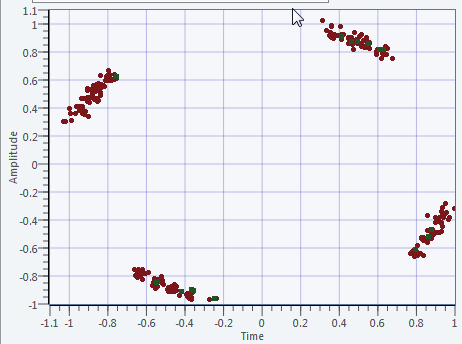
\includegraphics[scale=0.58]{img/multicarrier_200hz.png}
     \caption{OFDM with a frequency offset of 200 Hz}
     \label{fig6}
    \end{minipage}\hfill
    \begin{minipage}[b]{0.48\linewidth}
         \centering 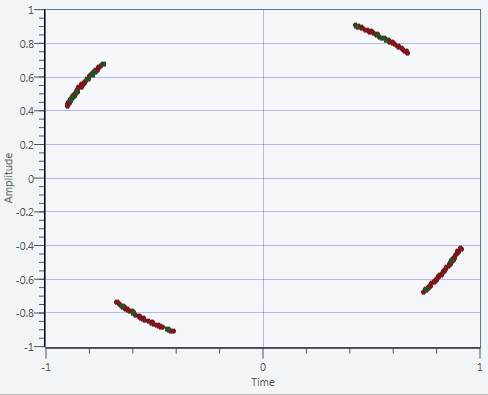
\includegraphics[scale=0.5]{img/SingleCarrier_Offset_200}
 \caption{Single-carrier systems with a frequency offset of 200 Hz}\label{fig7}
    \end{minipage}
\end{figure}

\begin{enumerate}

\item On the figure \ref{fig6}, we consider a OFDM system. Like, the channel response is frequency-selective, the attenuation is not the same on each symbol.

\item  On the figure \ref{fig7}, we have a single-carrier system, whith a constant attenuation, which can be seen on the figure by a aligned line.
\end{enumerate}

\subsection{What is the subcarrier spacing $\Delta_c$ of your system when $N = 1024$ and $64$ respectively?}

We use the following equation
\begin{equation}
\Delta_c=\frac{1}{NT}
\end{equation}
with T the sample period and N the FFT size. Finally, we obtain the following result

\begin{center}
	\begin{tabular}{c|c|c}
		  & $N=64$ & $N=1024$\\
		  \hline
	$\Delta_c$ & $\textbf{15625~kHz}$ & $\textbf{976.56 kHz}$ \\
	\end{tabular}
	\label{tab3}
\end{center}

As we can see with the value above, the subcarrier spacing is much larger in a narrowband channel then in a wideband channel. So, in the frequency domain, we have more inter carrier frequency in wideband then in narrowband because the symbols have less space for $N=1024$.

\subsection{Which of the systems (i.e., $N = 1024$ or $64$) is more severely impacted by a $200 Hz$ frequency offset? Why?}

The most impacted system is the one with $\textbf{N=1024}$. In fact, the symbols have less space in the frequency domain which cause a error called \textit{Inter Carrier Interference(ICI)}, and also phase shift. It is equivalent to the \textit{Inter Symbol Interference (ISI)} in single-carrier systems.

\subsection{Discuss this relationship between the effect of symbol timing error in single carrier systems and frequency offset in OFDM systems}

\begin{enumerate}
\item In single-carrier system, we have Inter Symbol Interference due to a \textbf{delay} introduced by the channel in the transmitted signal. The delay become a much bigger issue if the symbols are sent rapidly one after another. This introduced errors give rise to a rotation off all the symbols on the constellation of the same value.

\item In a multi-carrier System, we have the same kind of problem but in the frequency domain due to the \textbf{frequencies offsets} introduced by the channel, N times different. This gives rise to a rotation of the symbol, but all the symbol will not be modified by the same error. This is due to the fact that we don't have the same delay for all the sub-carriers.

\end{enumerate}

\section{More question}

\subsection{What is the effective data rate of the OFDM system in lab?}
%TODO answer to the question
The effective data rate of the OFDM system is given by the following formula
$$OFDM~symbol~rate = \frac{1/T}{(N + L_C + K)} $$
\subsection{Discuss why or why not you might use an OFDM system in a wideband and narrowband system respectively}

As deduced from the previous question, we know that a wideband system is frequency-selective and a narrowband system is flat. Like, an OFDM system is useful to devide a frequency-selective channel into N flat subchannels. Thus, an OFDM system will be used on a wideband channel instead of a narrowband channel.
However, the single-carrier system will be used on a flat channel, which corresponds to a narrowband channel.

\subsection{Name at least three parameters of OFDM systems which contribute to this flexibility and comment on how they do so}
%TODO add comment 
\begin{enumerate}
\item N This parameter modify the space in the frequency domain between symbols.   This space can cause an Inter Carrier Interference if it's too small.
\item $L_C$ This parameter modify the length cyclic prefix. When the length cyclic prefix is changed, the data rate of the OFDM system change. 
\item $1/T$ 
\end{enumerate}






\end{document}
